\documentclass[rapport.tex]{subfiles}
\begin{document}
\chapter*{\uppercase{Revue de la documentation}}
\addcontentsline{toc}{chapter}{REVUE DE LA DOCUMENTATION}
Afin de réaliser le projet, l’équipe de développement a dû faire des recherches préliminaires. Les technologies utilisées n’étaient pas maitrisées par l’équipe au démarrage du projet. Donc, les recueils de documentation et les projets exemples présents sur internet ont été une bonne source d’information.
\par
Cette section présentera donc ces ressources pour les grandes parties du projet, soit le périphérique Structure Sensor, la trousse de développement logiciel de réalité augmentée d'Apple et la gestion de projet.
\section*{Structure Sensor}
\addcontentsline{toc}{section}{Structure Sensor}
Occipital, la compagnie propriétaire du périphérique, publie régulièrement une version de leur trousse de développement logiciel exposant des interfaces de programmation. La dernière version publiée par la compagnie est la version 0.7.1 en février 2018. \citep*{occipitalsdk} La version du SDK étant inférieure à 1.0.0, on comprend que la première version complète est encore en développement.
\par
Dans l’état actuel, le SDK fournit quand même une liste d’interface disponible dans deux fichiers, Structure et StructureSLAM. Le premier est composé des différentes interfaces de contrôle du périphérique. Alors que le deuxième est un regroupement des classes permettant le contrôle des mailles en position tridimensionnelles et les textures de ceux-ci.
\par
Ces interfaces seront la base de la conception du module de prise de modèle grâce au périphérique. Les tâches de chacune des interfaces ont été identifiées lors de la lecture du code des entêtes des interfaces en Objective-C. L’équipe a produit un diagramme de classe afin d’améliorer la compréhension des responsabilités de chacune des interfaces et les relations entre celles-ci. Celui-ci est présenté à la page suivante.
\begin{figure}[H]
    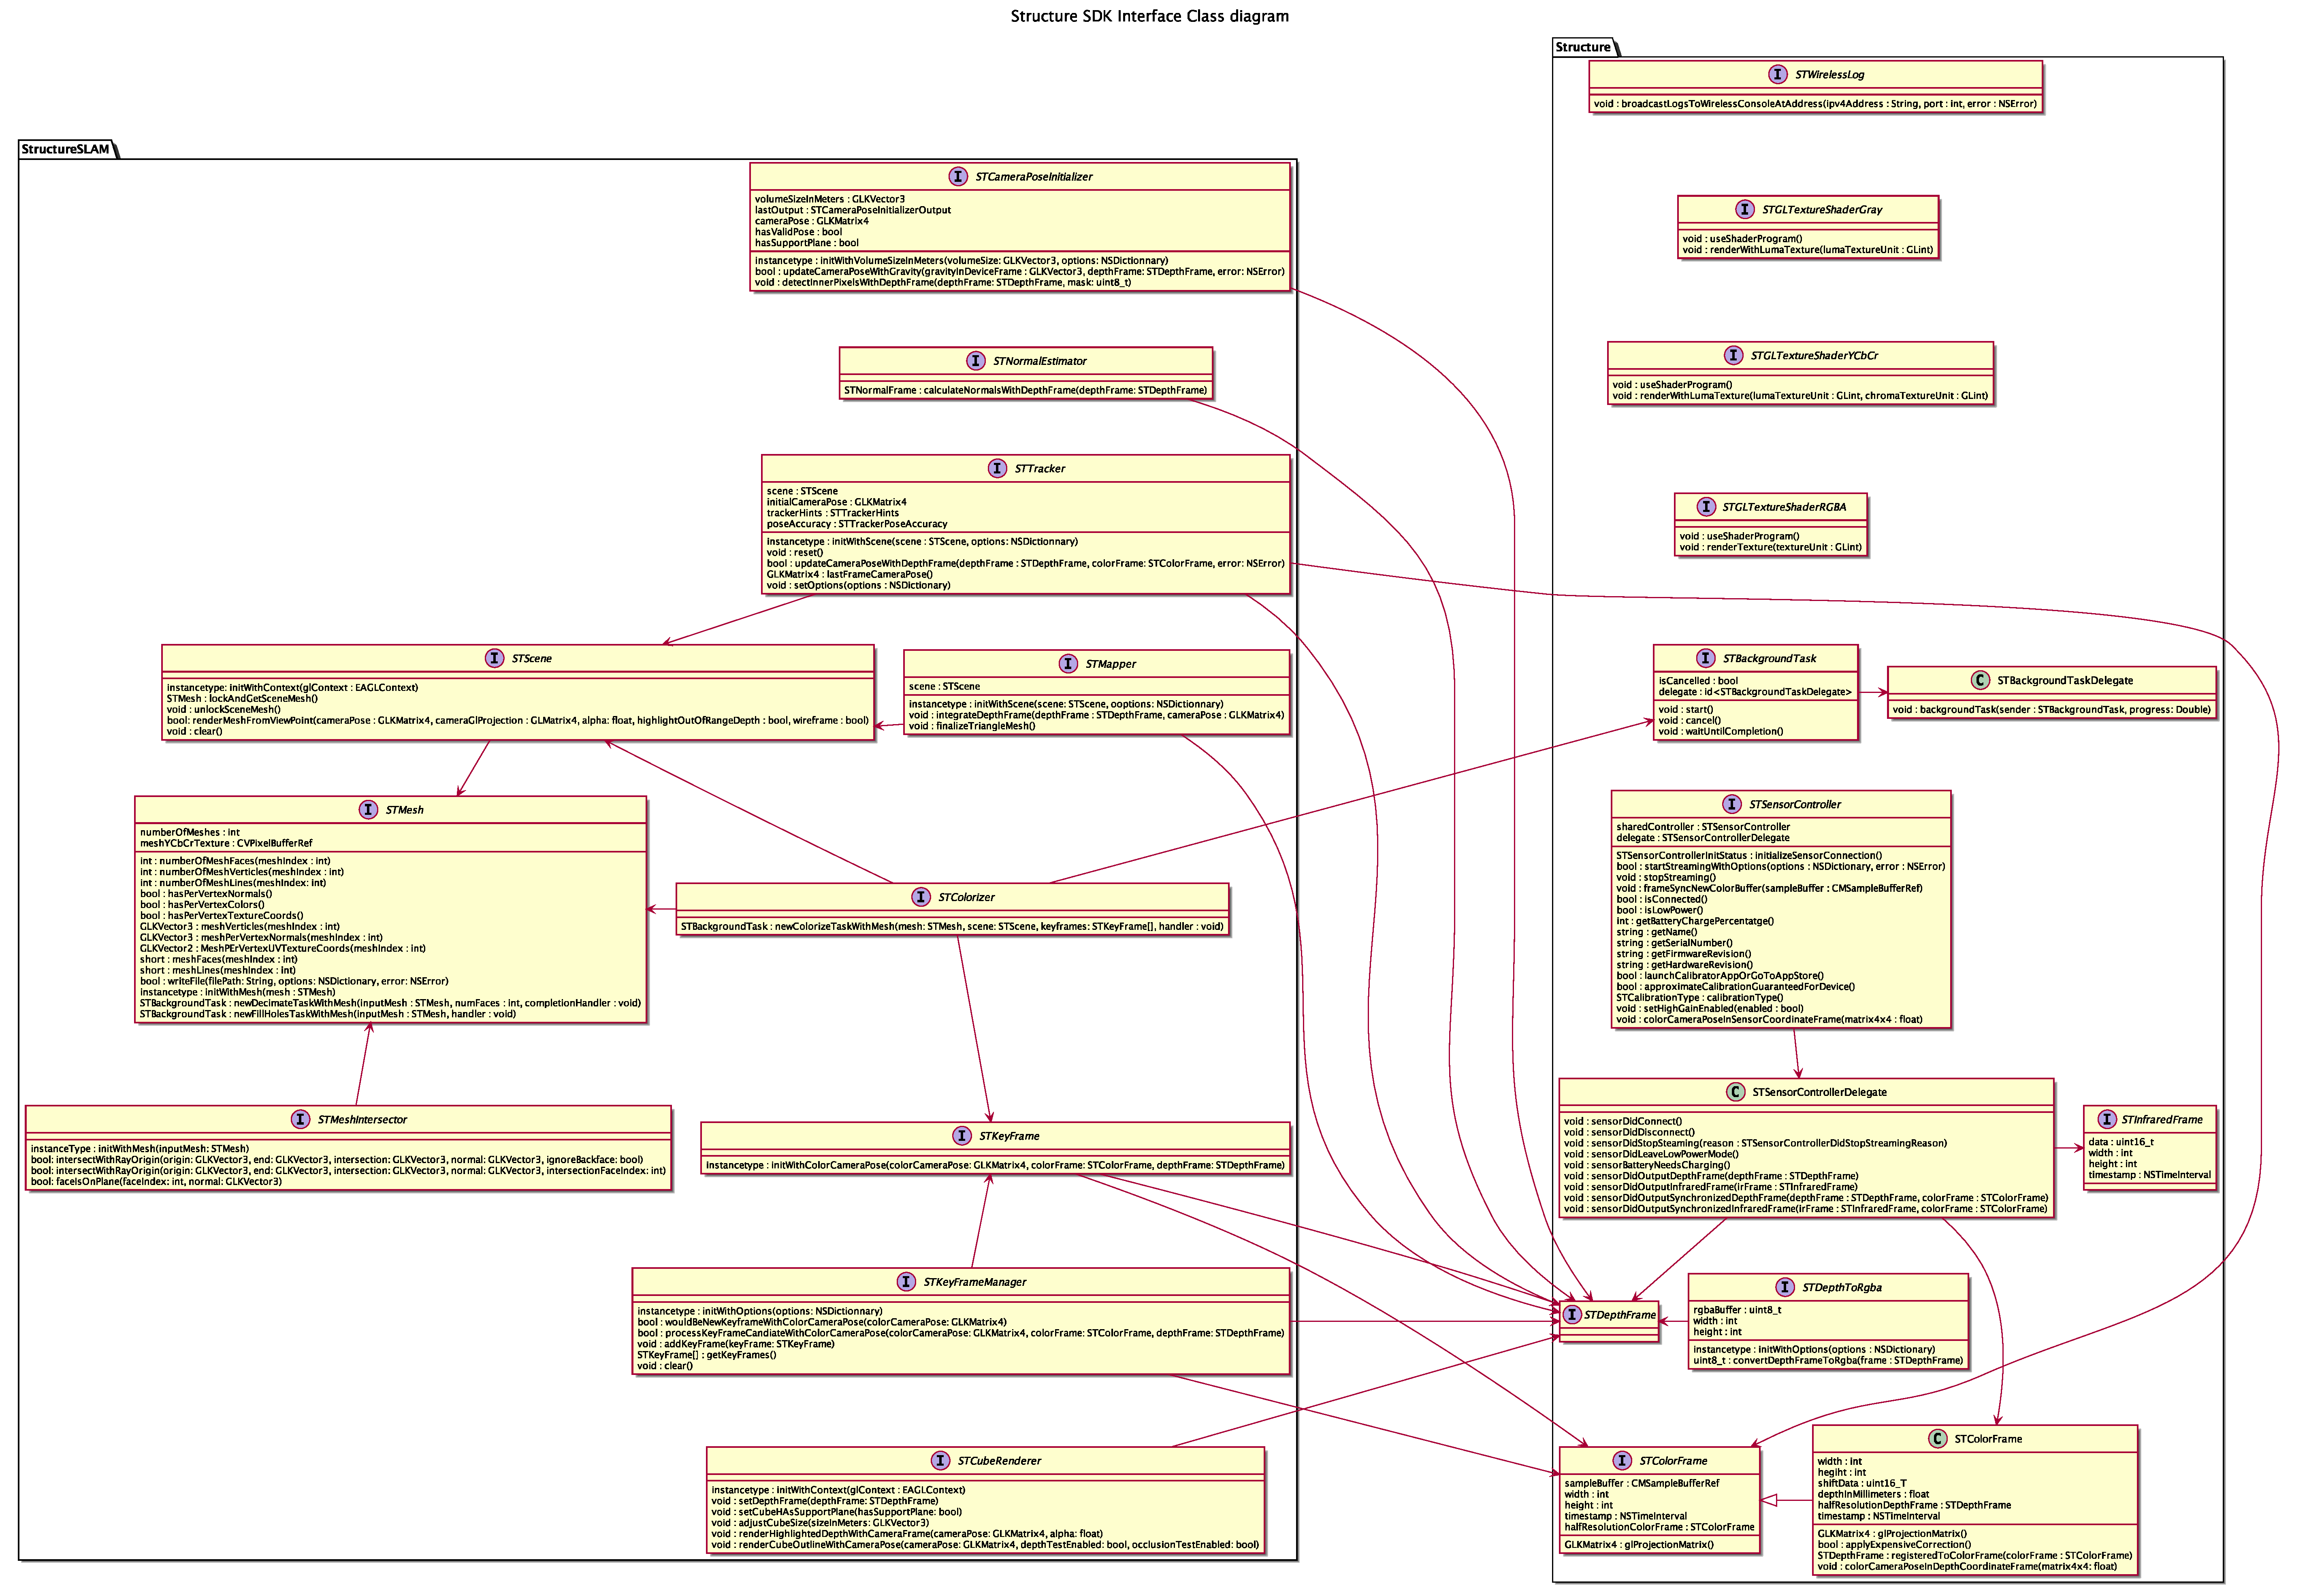
\includegraphics[width=.8\textheight, angle=90]{StructureClassDiagram.eps}
\centering
    \caption{Diagramme de classes du Structure Sensor SDK}
\end{figure}
Dans le diagramme, on constate que plusieurs patrons de conception ont été utilisés et exposés dans l’interface. La classe STSensorControllerDelegate servira de point d’ancrage entre notre application et le Structure Sensor. Cette interface permet donc de réduire les communications ou les recherches d’informations dans la logique d’affaires. La plupart de l’usage du SDK dans l’application devra être fait par cette classe.\citep*{bpse01} 
\par
Le Structure Sensor utilise les DepthFrame et ColorFrame pour comprendre l’environnement dans lequel il est utilisé. Ces concepts ont été introduits par Kinect un des premiers Senseurs 3D ayant connu un succès commercial étant donné son intégration dans l’environnement Xbox 360 de Microsoft. \citep*{microsoft01} 
\par
Le Structure SDK contient aussi plusieurs exemples d’application afin de guider les développeurs dans le développement de leurs applications. Le plus intéressant pour l’objectif du projet est le Scanneur. Celui-ci permet de convertir un objet dans l’espace de test en un modèle 3D et l’envoyer par courriel. D’autres fonctions incluses dans cet exemple sont la colorisation du modèle et les différentes options de capture. L’espace de capture est aussi indiqué par un cube et un plan utilisant les couleurs pour indiquer les objets qui peuvent être capturés.
\par
Les principales sections du SDK utilisé dans cet exemple sont le STStructureSensorDelegate pour le contrôle du périphérique. Les STDepthFrames et les STColorFrames ou en français les grilles de profondeurs et les grilles de couleurs permettant de créer le modèle STMesh. Une fois le modèle scanner en maille celui-ci est présenté dans le MeshViewController grâce au rendu de maille, STMeshRenderer. Le langage de programmation utilisé dans la globalité du SDK est l’Objective-C.
\par
Dans le but d’utiliser des technologies qui sont à jour avec les pratiques de l’industrie, l’équipe de développement souhaite utiliser le nouveau langage de programmation Swift. Celui-ci est le nouveau langage proposé par Apple pour le développement mobile. Le langage est déjà à sa quatrième version majeure et a pour but de simplifier la syntaxe qui était auparavant utilisée soit l’Objective-C.\citep*{swift01} Un membre de la communauté de développeur Structure a produit un port de l’exemple de Scanneur en Swift 2. L’équipe devra donc faire les changements nécessaires à cette version pour la compiler avec la version 4.\citep*{structureScannerSwift} 
\par
L’exemple de scanneur qui sera utilisé comme base du module de scan utilise plusieurs autres APIs par Apple. Ces APIs sont documentées sur le site de Apple dans la section pour développeurs. \citep{appleDev} L’équipe utilisera donc cette ressource en ligne pour accomplir la tâche.
\section*{Apple ARKit}
\addcontentsline{toc}{section}{Apple ARKit}
En juin 2017, Apple, une compagnie informatique californienne a lancé la 11e version de son système d’exploitation pour les développeurs. Cette nouvelle version apporte aux utilisateurs plusieurs nouvelles fonctionnalités, dont un gestionnaire de fichiers, appuyer fort sur une icône pour avoir plus d’options et aussi la possibilité d’apporter la réalité augmentée aux appareils mobiles. Il s’agit de la naissance de la librairie ARKit de Apple. \citep{cloverJ01}
\par
Apple a créé l’ARKit en voyant le marché émergent des jeux en réalité augmentée depuis les dernières années. Le problème avec ces jeux c’est qu’il faut avoir un ordinateur très performant pour pouvoir y jouer. En apportant de la réalité augmentée aux appareils mobiles, Apple rend plus abordable ce genre de jeux et offre de belles possibilités aux développeurs.
\par
Cette librairie utilise l’algorithme SLAM (Simultaneous Localization and Mapping) afin de se retrouver dans l’espace. Cet algorithme est utilisé dans les robots ou véhicules autonomes. Il sert à créer une carte virtuelle de l’environnement réel. Une fois cette carte générée, l’algorithme la garde à jour et garde le positionnement de l’appareil dans l’environnement. C’est grâce à cet algorithme qu’il est possible de donner des coordonnées cartographiques à un modèle généré par ordinateur et de l’apercevoir dans l’environnement réel. \citep*{Thrun2008}
\par
De plus, l’apprentissage de l’ARKit se fait très bien, le site d’Apple possède une grande quantité de documentation sur chaque fonction provenant de la librairie et il existe une grande variété d’exemples pour comprendre l’utilisation. Cette librairie est disponible dans le nouveau langage Swift d’Apple et dans l’ancien qui est l’objective-c. L’équipe a choisi d’utiliser la version la plus récente de Swift pour éviter des problèmes discontinuités.
\end{document}
